\section{Anwendungsschicht}

\paragraph{Historie}
\begin{items}
  \item \textbf{70er/80er}: \\*
    - textbasierte Anwendungen
  \item \textbf{90er}: \\*
    - World Wide Web \\*
    - Instant Messaging \\*
    - P2P-Filesharing
  \item \textbf{seit 2000}: steigende Vielfalt + Allgegenwärtigkeit \\*
    - Streaming (Spotify, YouTube) \\*
    - Gaming \\*
    - Soziale Netzwerke \\*
    - Smartphones
\end{items}

\paragraph{Grundlagen --- Schichtenmodell}
\begin{items}
  \item Kommunikation in Schichten organisiert
  \item \textbf{Anwendungsschicht}: oberste Schicht \\*
    - enthält Anwendungsprotokolle \\*
    - Anwendung kümmert sich nicht um Datentransport
  \item \textbf{Datentransport}: unter Anwendungsschicht liegende Schichten \\*
    - Interna für Anwendung transparent \\*
    - Verzögerungen bleiben vor Anwendung verborgen
\end{items}

\paragraph{Grundlagen --- Verzögerung}
\begin{items}
  \item Abhängig von \\*
    - \emph{Ausbreitungsverzögerung} \( t_a \) \\*
    - \emph{Sendezeit} \( t_s \) \\*
    - \emph{Pufferfüllstände}
  \item \textbf{Ausbreitungsverzögerung} \( t_a = \tfrac{d}{v} \) \\*
    - \emph{Zeitspanne zwischen Absenden eines Signals und dessen Eintreffen am anderen \\* \phantom{-} Ende des Mediums} \\*
    - Abhängig von: \\* 
      \phantom{-} Ausbreitungsgeschwindigkeit \( v \) \\*
      \phantom{-} Länge des Mediums \( d \)
  \item \textbf{Sendezeit} \( t_s = \tfrac{X}{r} \) \\*
    - \emph{Zeit zwischen Beginn und Abschluss der Sendung} \\*
    - Abhängig von: \\*
      \phantom{-} Datenmenge \( X \) \\*
      \phantom{-} Datenrate des Mediums \( r \) \\*
    - \textbf{Achtung}: Nach Sendungsabschluss sind die Daten noch nicht beim Empfänger! \\* \phantom{-} \( \leadsto \) Ausbreitungsverzögerung \( t_a \)
  \item \textbf{Verzögerung im Router} \\*
    - \emph{Pufferung} der Daten in Warteschlange \\*
    - \emph{Verarbeitung} (Fehlerüberprüfung usw.)
\end{items}

\paragraph{Grundlagen --- Protokollstack}
\begin{items}
  \item \textbf{Application}: SMTP, HTTP, XMPP,\dots
  \item \textbf{Transport}: TCP, UDP
  \item \textbf{Network}: IP
  \item \textbf{Data Link}: Ethernet, 802.11 (WiFi)
  \item \textbf{Physical}: Bits auf Medium
\end{items}

\paragraph{Grundlagen --- Prozess und Nachricht}
\begin{items}
  \item \textbf{Prozess}: Programm, das im Endsystem (Anwendungsschicht) abläuft
  \item \textbf{Nachricht}: Ausgetauscht zwischen Prozessen auf \emph{unterschiedlichen} Endsystemen
\end{items}

\paragraph{Grundlagen --- Socket und Interface}
\begin{items}
  \item \emph{Programmierschnittstelle für verteilte Anwendungen}
  \item Von OS bereitgestellte API
  \item Anwendungsprozess sendet/empfängt Nachrichten zum/vom Socket
  \item \textbf{Portnummern}: (De-) Multiplexing auf Endsystemen \\*
    - viele Prozesse auf Endsystem kommunizieren gleichzeitig über Netzwerk \\*
    \phantom{-} \( \leadsto \) eindeutige Socket-Identifikation über Portnummer
\end{items}

\paragraph{Grundlagen --- Client-Server-Anwendungen}
\begin{items}
  \item \textbf{Server}: \\*
    - ständig in Betrieb \\*
    - permanente IP-Adresse \\*
    - häufig in Datenzentren
  \item \textbf{Clients}: \\*
    - kommunizieren mit Server \\*
    - kommunizieren \emph{nicht} direkt miteinander \\*
    - evtl. nicht immer verbunden \\*
    - evtl. dynamische IP-Adresse
\end{items}

\paragraph{Grundlagen --- Peer-to-Peer-Anwendungen}
\begin{items}
  \item Endysteme kommunizieren direkt miteinander \\*
    - fordern Dienste von anderen Peers an \\*
    - nicht permanent verbunden, wechseln dymanisch IP-Adressen \\*
    \phantom{-} \( \leadsto \) komplexes Management
  \item selbst-skalierend \\*
    - neue Peers erhöhen Kapazität, fordern aber auch selber Dienste an
\end{items}

\paragraph{Web und HTTP --- Web-Dokumente}
\begin{items}
  \item Webseiten bestehen aus Basis-HTML-Datei und anderen Objekten (.js, .png,\dots)
  \item Jedes Objekt über URL (\emph{uniform resource locator}) referenzierbar
\end{items}

\paragraph{HTTP --- Überblick}
\begin{items}
  \item Protokoll der Anwendungsschicht (\emph{hypertext transfer protocol}) \\*
    - einfaches, ASCII-basiertes Transferprotokoll
  \item Basiert auf Client/Server-Modell \\*
    - \emph{Client}: Browser, der Web-Objekte anfordert, empfängt und darstellt \\*
    - \emph{Server}: sendet über HTTP angeforderte Objekte
  \item zwei Nachrichten-Typen: \emph{Request}, \emph{Response}
  \item Zustandslos: \\*
    - jeder Request wird individuell bearbeitet \\*
    - keine Zustandsinformation auf dem Server
  \item nutzt TCP zur Kommunikation \\*
    1. Client initiiert Verbindungsaufbau \\*
    2. Server akzeptiert Verbindung \\*
    3. Austausch von HTTP-Nachrichten \\*
    4. Abbau der TCP-Verbindung
\end{items}

\paragraph{HTTP --- Methoden}
\begin{items}
  \item \emph{HTTP-Anfragen können verschiedene Methoden nutzen}
  \item \textbf{GET}: Resource von Server zu Client übertragen (z.B. normale Webseite)
  \item \textbf{POST}: Daten zu Ressource übertragen (z.B. Web-Formular)
  \item Weitere Methoden: \\*
    - PUT --- neue Ressource anlegen \\*
    - DELETE --- Ressource löschen \\*
    - HEAD --- wie GET, aber nur HTTP-Header übertragen \\*
    - \dots
\end{items}

\paragraph{HTTP --- Status-Codes}
\begin{items}
  \item Verarbeitungsindikator (Erfolg/Fehlschlag + Gründe)
  \item \textbf{200}: Erfolg; Antwort ist in dieser Nachricht
  \item \textbf{301}: Angefragtes Objekt wurde verschoben (neue URL in Nachricht spezifiziert)
  \item \textbf{400}: Server hat Anfrage nicht verstanden
  \item \textbf{404}: Angefordertes Objekt existiert nicht
  \item \textbf{505}: HTTP-Version nicht unterstützt
\end{items}

\paragraph{HTTP --- Verbindungen}
\begin{items}
  \item \textbf{Non-persistent HTTP}: \\*
    - höchstens ein Objekt wird über TCP-Verbindung gesendet, danach geschlossen \\*
    \phantom{-} \( \leadsto \) Herunterladen mehrerer Objekte erfodert mehrere TCP-Verbindungen
  \item \textbf{Persistent HTTP}: mehrere Objekte über eine TCP-Verbindung
\end{items}

\paragraph{Non-persistent HTTP --- Antwortzeit}
\begin{items}
  \item \textbf{Round Trip Time (RTT)}: Zeit, die Paket von Sender zu Empfänger und zurück benötigt
  \item \textbf{HTTP-Antwortzeit}: \\*
    - ein RTT für Verbindungsaufbau \\*
    - ein RTT für HTTP-Anfrage und erste Antwortbytes \\*
    - Zeit \( t_s \) für Senden der Datei \\*
    \phantom{-} \( \leadsto \) \textbf{Antwortzeit} \( 2*\text{RTT} + t_s \) 
\end{items}

\paragraph{Cookies}
\begin{items}
  \item \emph{Speichert Nutzer-Server-Zustand}
  \item \( \leadsto \) Server kann Inhalt abhängig von Nutzeridentifikation bereitstellen
  \item \textbf{Komponenten}: \\*
    - Cookie-Information in HTTP-Response-Nachricht \\*
    - Cookie-Information wird in nachfolgenden HTTP-Requests genutzt \\*
    - Datei mit Cookies wird auf Nutzer-Endsystem vom Browser verwaltet \\*
    - Datenbank bei Webseite \( \leadsto \) Server muss Cookies richtig interpretieren können
\end{items}

\paragraph{Cookies --- Privatsphäre}
\begin{items}
  \item Webseiten unterscheiden Nutzer durch Cookies \\*
    \( \leadsto \) Werbeanbieter können Nutzer über viele Webseiten tracken
  \item Webseiten können durch Cookies sehr viel über Nutzer lernen
\end{items}

\paragraph{Mail --- Komponenten}
\begin{items}
  \item \textbf{User Agent} (UA): \\*
    - lesen, senden, weiterleiten \\*
    - Beispiele: Outlook, Thunderbird
  \item \textbf{Mailserver}: \\*
    - \emph{mail transfer agent} (MTA) \\*
    - \emph{mail delivery agent} (MDA) \\*
    - User-Mailboxen
  \item \textbf{\emph{simple mail transfer protocol}} (SMTP) \\*
    - Client/Server-Modell \\*
    - Transfer von Mails vom User Agent zum Mailserver
\end{items}

\paragraph{SMTP --- Aufbau}
\begin{items}
  \item Drei Phasen: \\*
    1. Handshake \\*
    2. Nachrichtenübermittlung \\*
    3. Abschluss
  \item Command/Response-Interaktionen \\*
    - ähnlich Request/Response bei HTTP \\*
    - Kommandos: ASCII-Text \\*
    - Antwort: Statuscode + Nachricht
\end{items}
\begin{figure}[H]\centering\label{SMTPAufbau}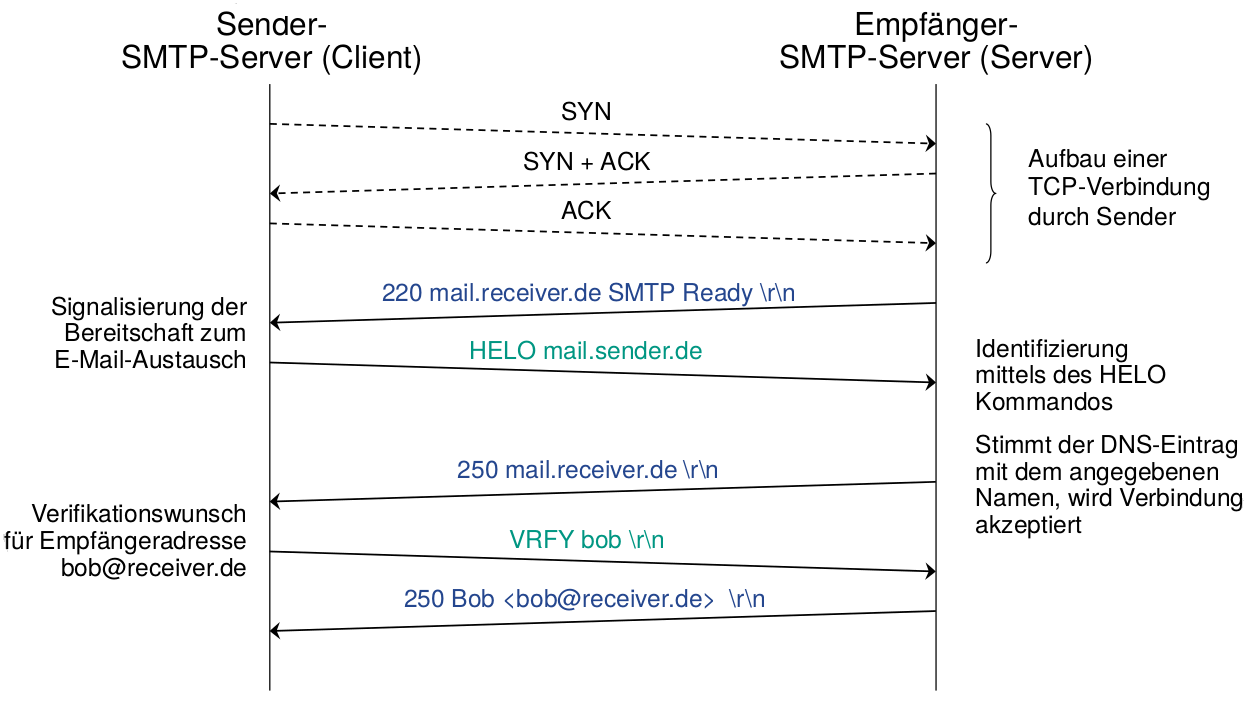
\includegraphics[width=0.33\textwidth]{SMTPAufbau}\end{figure}

\paragraph{MIME}
\begin{items}
  \item \textbf{Problem}: SMTP kann nur ASCII-Texte versenden, keine Dateien
  \item \textbf{MIME}: erweitert Kopfteil einer Nachricht um Formatinformation \\*
    - \emph{Content-Type}: Definiert Typ des E-Mail-Inhalts
\end{items}

\paragraph{Mail --- Postfach-Abfrage}
\begin{items}
  \item \textbf{POP3} (\emph{post office protocol 3}): \\*
    - Client holt von Mailserver empfangene/gespeicherte Nachrichten ab \\*
    - einfache Funktionalität \\*
    - verwaltet Nachrichten im UA, \emph{keine} Synchronisation zwischen mehreren UAs
  \item \textbf{IMAP} (\emph{interactive mail access protocol}): \\*
    - Nachtichten werden zentral auf Mailserver verwaltet \\*
    - erweiterte Kommandos (Ordner, Filter) \\*
\end{items}

\paragraph{XMPP}
\begin{items}
  \item \emph{Echtzeit-XML-Streaming-Protokoll}
  \item Grundlage für Whatsapp usw.
  \item Dezentral, ähnlich wie E-Mail
  \item \textbf{Clients}: zu ihrem jeweiligen Server verbunden
  \item \textbf{Server}: verbinden sich untereinander zur Nachrichtenübermittlung
  \item \textbf{Adressformat}: \\*
    - \emph{Nutzer}: Server + Username, z.B. alice@jabber.org \\*
    - \emph{Clients}: pro Nutzer, z.B. alice@jabber.org/laptop
\end{items}

\paragraph{DNS --- Grundlagen}
\begin{items}
  \item \textbf{Ziel}: Verwendung von Namen statt IPs
  \item \textbf{Aufgabe}: Zuordnung IP-Adresse \( \leftrightarrow \) Name
  \item \textbf{Funktionalitäten}: \\*
    - \emph{Registrierung} von Namen + IP-Adressen \\*
    - \emph{Auflösung} von Namen in IP-Adressen
\end{items}

\paragraph{DNS --- Aufbau}
\begin{items}
  \item Verteilte Datenbank von Name-Servern (DNS-Servern) \\*
    - Client-Server-Modell \\*
    - Server kann Anfrage an weitere Server weiterleiten
  \item Protokoll der Anwendungsschicht \\*
    - Über Port 53 (UDP) realisiert \\*
  \item Basisdienst \( \leadsto \) keine Anwendung \\*
    - Komplexität am Rande des Netzes lokalisiert \\*
    \phantom{-} \( \to \) Internet-Design-Philoshopie!
\end{items}

\paragraph{DNS --- Anfragen}
\begin{items}
  \item \textbf{Rekursiv}: kennt angefragter Server Antwort nicht, fragt dieser dahinterliegende Server, bis er Antwort bekommt
  \item \textbf{Iterativ}: kennt angefragter Server Antwort nicht, fragt \emph{Client} andere Server
  \item \textbf{Üblich}: Client fragt lokalen Name-Server rekursiv, dieser dann iterativ
\end{items}

\paragraph{DNS --- Resource Records (RR)}
\begin{items}
  \item DNS ordnet Domänen zu Einträgen zu
  \item \textbf{A / AAAA} (Adress): Abbildung Name auf IPv4/IPv6-Adresse
  \item \textbf{MX} (Mail Exchange): Mailserver einer Domäne
  \item \textbf{NS} (Name Server): Nameserver einer Domäne
  \item \textbf{CNAME} (Canonical Name): Alias-Namen für Rechner/Domänen
  \item \textbf{PTR} (Pointer): Abbildung IP-Adresse auf Name
\end{items}